\documentclass[12pt,a4paper,ngerman]{article}
\usepackage{stylesheet}
\usepackage{epstopdf}
\begin{document}

\TUHeader                          %  Bitte Ausfüllen!!!
%----------------------------
{Übung F: Übertragungsverhalten nachrichtentechnischer Systeme}                       %  Übungstitel
%----------------------------
{25.11.2014}                        %  Übungsdatum
%----------------------------
{05}                            %  Gruppen-Nr.
%----------------------------
{Thomas Neff}                   % Name des Protokollführers
%----------------------------
{
1.~Daniel Freßl, 1230028\\
2.~Thomas Neff, 1230319\\                    %  Übungsteilnehmer
3.~Thomas Pichler, 1230320 \\                   %  ...bei <4 Teilnehmer auskommentieren
4.~Martin Winter, 1130688\\
5.~Bernadette Schreyer, 1073076\\
}
%----------------------------
{Ao.Univ.-Prof. Dipl.-Ing. Dr. techn. Erich Leitgeb}
{Max Henkel}                          %  Betreuer
%----------------------------
{Graz}                              %  Ort der Protokollerstellung
{\today}                            %  Datum Protokollerstellung




\pagebreak
  
\tableofcontents
  
\pagebreak

%-------------------------------------------------------------------------------
%
% Beginn des Protokolls
%
%-------------------------------------------------------------------------------

\section{Analyse eines unbekannten Filters}
\subsection{Aufgabenstellung}
In dieser Aufgabe soll das Verhalten eines unbekannten Filters untersucht werden. Zuerst soll eine grundsätzliche Aussage über die Art und Ordnung des Filters getroffen und danach das Filter so eingestellt werden, dass am Ausgang maximales Überschwingen beobachtet werden kann. 
Die Eigenfrequenz dieser Konfiguration ist zu bestimmen. Weiters soll ein Bodediagramm bei einer Einstellung mit 60\% Überschwingen aufgenommen und das System durch einen äquivalenten RLC-Serienschwingkreis ersetzt werden. Dazu wird der Widerstand gemessen und L, C berechnet.

\subsection{Messaufbau}

Das unbekannte System wurde mit Hilfe eines Frequenzgenerators gespeist und die folgenden Messungen mit Hilfe eines analogen Oszilloskops gemessen. 

\subsection{Tabellen}
\begin{table}[H]
\begin{center}
\begin{tabular}{ |c|c||c|c||c|c| }
  \hline
    $\frac{T}{2}_{Scale}$ & $\frac{T}{2}_{Div}$ & $\delta$t$_{Scale}$ & $\delta$t$_{Div}$ & $U_{a,Scale}$ & $U_{a,Div}$\\

    [$\frac{ms}{Div}$] & [Div] & [$\frac{ms}{Div}$] & [Div] & [$\frac{V}{Div}$] & [Div]\\
  \hline
$5$ & $4.6$ & $0.5$ & $0.7$ & $0.5$ & $4.0$ \\
  \hline
$0.5$ & $5.8$ & $0.5$ & $0.4$ & $0.5$ & $5.0$ \\
  \hline
$0.2$ & $6.8$ & $0.2$ & $3.4$ & $1.0$ & $6.0$ \\
  \hline
$0.2$ & $5.0$ & $0.2$ & $4.2$ & $0.5$ & $4.1$ \\
  \hline
$0.1$ & $5.0$ & $0.1$ & $4.7$ & $0.05$ & $6.4$ \\
  \hline
\end{tabular}
\caption{Gemessene halbe Periodendauer, Phasenverschiebung und Ausgangsspannung bei verschiedenen Frequenzen.}
\end{center}
\label{tab:1}
\end{table}

\begin{table}[H]
\begin{center}
\begin{tabular}{ |c|c|c|c|c|c|c| }
  \hline
    T & $\delta$t & $U_a$ & f & $\phi$ & A & $A_{dB}$\\

    [ms] & [ms] & [V] & [Hz] & [$^\circ$] & & [dB]\\
  \hline
$46$ & $0.35$ & $2$ & $21.74$ & $-2.74$ & $1$ & $0$\\
  \hline
$5.8$ & $0.2$ & $2.5$ & $172.41$ & $-12.4$ & $1.25$ & $1.94$\\
  \hline
$2.72$ & $0.68$ & $6$ & $367.65$ & $-90$ & $3$ & $9.54$\\
  \hline
$2$ & $0.84$ & $2.05$ & $500$ & $-151.2$ & $1.025$ & $0.21$\\
  \hline
$1$ & $0.47$ & $0.32$ & $1000$ & $-169.2$ & $0.16$ & $-15.92$\\
  \hline
\end{tabular}
\caption{Berechnete Periodendauer, Phasenverschiebung in ms und Grad, Ausgangsspannung, Frequenz und Verstärkung.}
\end{center}
\label{tab:1_ber}
\end{table}

\subsection{Formeln}
Die Periodendauer T ergibt sich aus
\begin{equation}
T = 2 \cdot \frac{T}{2}_{Scale} \cdot \frac{T}{2}_{Div}
\end{equation}
Die Phasenverschiebung $\delta$t in ms ergibt sich durch
\begin{equation}
\delta t = \delta t_{Scale} \cdot \delta t_{Div}
\end{equation}
Die Ausgangsspannung $U_a$ wird mit
\begin{equation}
U_a = U_{a,Scale} \cdot U_{a,Div}
\end{equation}
berechnet.
Die Frequenz f berechnet man mit
\begin{equation}
f = \frac{1}{T}
\end{equation}
Die Phasenverschiebung $\phi$ in $^\circ$ ergibt sich durch
\begin{equation}
\phi = - \frac{\delta t}{T} \cdot 360^\circ
\end{equation}
Die Verstärkung A berechnet man mit
\begin{equation}
A = \frac{U_a}{U_e}
\end{equation}\\
Die Verstärkung $A_{dB}$ berechnet man mit
\begin{equation}
A_{dB} = 20 \cdot log(A)
\end{equation}
Als Ersatzschaltung für den unbekannten Filter wurde ein RLC-Serienschwingkreis mit der Abnahme von $U_a$ über C verwendet. Die Formeln wurden vom Betreuer angegeben.
Die Übertragungsfunktion der Ersatzschaltung lautet
\begin{equation}
G(s) = \frac{1}{s^2 LC + sRC + 1}
\end{equation}
Die Induktivität L wurde mit folgender Formel berechnet.
\begin{equation}
L = \frac{R}{2 \zeta \omega_n}
\end{equation}
Die Kapazität C berechnet man mit 
\begin{equation}
C = \frac{1}{\omega_n^2L}
\end{equation}

\subsection{Berechnungsbeispiele}
Für die folgenden Berechnungsbeispiele wurden die Werte aus der ersten Zeile der Tabelle \ref{tab:1} verwendet.

\begin{equation}
T = 2 \cdot \frac{T}{2}_{Scale} \cdot \frac{T}{2}_{Div} = 2 \cdot 5\frac{ms}{Div} \cdot 4.6 Div = 46ms
\end{equation}
\begin{equation}
\delta t = \delta t_{Scale} \cdot \delta t_{Div} = 0.5\frac{ms}{Div} \cdot 0.7Div = 0.35ms
\end{equation}
\begin{equation}
U_a = U_{a,Scale} \cdot U_{a,Div} = 0.5\frac{V}{Div} \cdot 4.0Div = 2V
\end{equation}
\begin{equation}
f = \frac{1}{T} = \frac{1}{46ms} = 21.74Hz
\end{equation}
\begin{equation}
\phi = - \frac{\delta t}{T} \cdot 360^\circ = -\frac{0.35ms}{46ms	} \cdot 360^\circ = -2.74^\circ
\end{equation}\\
Als Eingangssignal wurde für die Aufnahme des Bodediagramm ein Sinussignal mit Spitze-Spitze-Spannung $U_e = 2V$ verwendet.
\begin{equation}
A = \frac{U_a}{U_e} = \frac{2V}{2V} = 1
\end{equation}
\begin{equation}
A_{dB} = 20 \cdot log(A) = 20 \cdot log(1) = 0 dB
\end{equation}
\\
Für die Berechnung der Bauteilwerte wurde als Ersatzschaltung ein RLC-Serienschwingkreis mit der Abnahme von $U_a$ über C verwendet. Der gemessene Widerstand des Filters betrug $R = 12.63k\Omega$. \\
Weiters wurde der vom Betreuer angegebene Wert für $\zeta \approx 0.16$ (für 60\% Überschwingen) und der Zusammenhang $\omega_n = 2 \pi f_n = 2 \pi \cdot 367.647Hz = 2310\frac{rad}{s}$ mit der gemessenen Eigenfrequenz $f_n = 367.647Hz$ verwendet.
\begin{equation}
L = \frac{R}{2 \zeta \omega_n} = \frac{12.63k\Omega}{2 \cdot 0.16 \cdot 2310\frac{rad}{s}} = 17.09H
\end{equation}
\begin{equation}
C = \frac{1}{\omega_n^2L} = \frac{1}{(2310\frac{rad}{s})^2 \cdot 17.09H} = 11pF
\end{equation}

\subsection{Diagramme}
\begin{figure}[H]
\centering
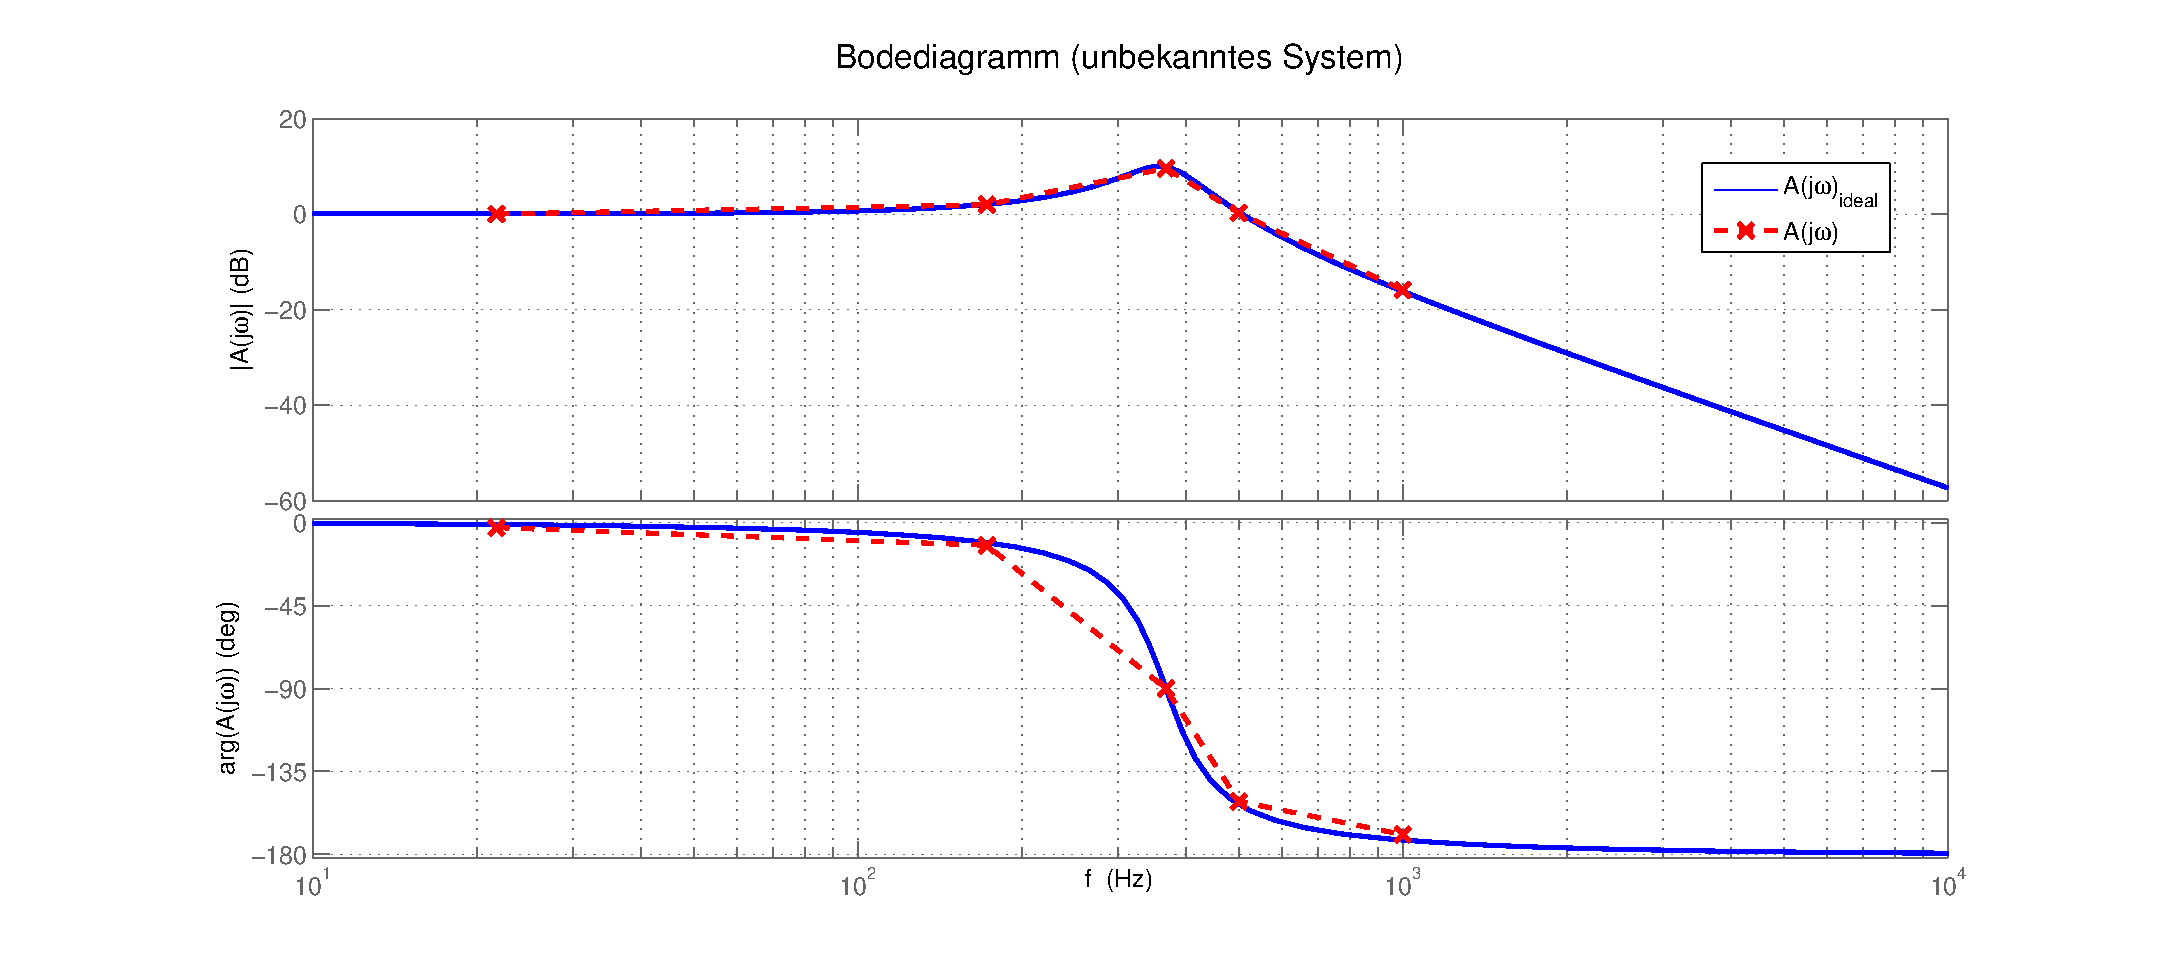
\includegraphics[width=1.2\textwidth]{figures/bode_unbekannt.eps} 
\caption{Bodediagramm des unbekannten Filters mit idealer und gemessener Kennlinie.}
\label{fig:bode_unb}
\end{figure}


\subsection{Geräteliste}
Neben dem AMREL FG-513 Funktionsgenerator und dem Voltcraft 662 Oscilloskop wurde auch ein Techtron DT-20 Multimeter verwendet.
\subsection{Diskussion}

Zunächst wurde mit Hilfe des Funktionsgenerators die Ausgangsspannung bei verschiedenen Frequenzen beobachtet. Hierbei konnten wir erkennen, dass die Phasenverschiebung bei zunehmender Frequenz stieg und die Amplitude sank. Da die Phasenverschiebung bei 3kHz $-180^\circ$ erreichte und sich Tiefpassverhalten ablesen ließ, muss es sich um einen Tiefpass 2. Ordnung gehandelt haben.
Um die Eigenfrequenz bei maximalen Überschwingen zu messen, wurde ein Rechtecksignal mit kleiner Frequenz ($5.6$Hz) eingespeist. Durch Überlagerung der einzelnen Schwingungsperioden des Überschwingens und dem Ausnützen des Nachleuchten des analogen Oszilloskops konnte eine Periodendauer von $2.72$ms abgelesen und ein Wert für die gedämpfte Eigenfrequenz von $f_n = 367.647$Hz errechnet werden. Diese wurde für die weiteren Schritte als die ungedämpfte Eigenfrequenz angenommen.
Die benötigten 60\% Überschwingen wurden mit den Potentiometern am Filter und der Prozentskala am Oszilloskop eingestellt. Mit dieser Einstellung wurde das Bodediagramm aufgenommen.\\
Im letzten Schritt wurde erklärt, das das System, obwohl es nicht bekannt ist, mit einer Ersatzschaltung mit ähnlichem Verhalten (Tiefpassverhalten 2.Ordnung und Schwingungsfähig) und der in Formel 8 gegebenen Übertragungsfunktion angenähert bzw. beschrieben werden kann. In diesem Fall wurde als Ersatzschaltung eine RLC-Serienschaltung mit der Abnahme von $U_a$ über dem Kondensator C verwendet. Hierfür wurden der Widerstand des unbekannten Filters gemessen ($R = 12.63k\Omega$) und die Bauteilwerte der Spule ($L = 17.09H$) und Kapazität ($C = 11nF$) berechnet. Mit diesen Werten wurde der ideale Frequenz- und Phasengang in der Abbildung \ref{fig:bode_unb} gezeichnet. Wie aus Abbildung \ref{fig:bode_unb} zu entnehmen ist, liegen die von uns gemessenen Werte sehr gut auf der idealen Kurve.



\pagebreak
\section{Analyse eines RC-Tiefpass-Filters}
\subsection{Aufgabenstellung}
Für einen RC-Tiefpass Filter mit den gegebenen Bauteilwerten $R = 13k\Omega$ und $C = 100 nF$ soll die Grenzfrequenz berechnet und gemessen werden, sowie das Bodediagramm aufgenommen werden.

\subsection{Messaufbau}
Das bekannte System wurde mit Hilfe eines Frequenzgenerators gespeist und die Eigenschaften mit Hilfe eines analogen Oszilloskops gemessen.

\subsection{Tabellen}
\begin{table}[H]
\begin{center}
\begin{tabular}{ |c|c||c|c||c|c| }
  \hline
    $\frac{T}{2}_{Scale}$ & $\frac{T}{2}_{Div}$ & $\delta$t$_{Scale}$ & $\delta$t$_{Div}$ & $U_{a,Scale}$ & $U_{a,Div}$\\

    [$\frac{ms}{Div}$] & [Div] & [$\frac{ms}{Div}$] & [Div] & [$\frac{V}{Div}$] & [Div]\\
  \hline
$2.0$ & $5.0$ & $2.0$ & $0.6$ & $0.5$ & $4.4$ \\
  \hline
$0.5$ & $9.1$ & $0.5$ & $2.3$ & $0.5$ & $3.6$ \\
  \hline
$0.5$ & $7.6$ & $0.5$ & $2.1$ & $0.2$ & $8.2$ \\
  \hline
$0.2$ & $4.7$ & $0.2$ & $2.0$ & $0.1$ & $5.0$ \\
  \hline
$0.02$ & $4.4$ & $0.02$ & $2.0$ & $0.01$ & $4.8$ \\
  \hline
$0.001$ & $4.7$ & $0.002$ & $1.1$ & $0.001$ & $2.8$ \\
  \hline
\end{tabular}
\caption{Gemessene halbe Periodendauer, Phasenverschiebung und Ausgangsspannung bei verschiedenen Frequenzen.}
\end{center}
\label{tab:2}
\end{table}

\begin{table}[H]
\begin{center}
\begin{tabular}{ |c|c|c|c|c|c|c| }
  \hline
    T & $\delta$t & $U_a$ & f & $\phi$ & A & $A_{dB}$\\

    [ms] & [ms] & [V] & [Hz] & [$^\circ$] & & [dB]\\
  \hline
$20$ & $1.2$ & $2.2$ & $50$ & $-21.6$ & $0.88$ & $-1.1$\\
  \hline
$9.1$ & $1.15$ & $1.8$ & $109.9$ & $-45.5$ & $0.72$ & $-2.85$\\
  \hline
$7.6$ & $1.05$ & $1.64$ & $131.58$ & $-49.7$ & $0.66$ & $-3.61$\\
  \hline
$1.88$ & $0.4$ & $0.5$ & $531.91$ & $-76.6$ & $0.2$ & $-13.98$\\
  \hline
$0.176$ & $0.04$ & $0.048$ & $5681.8$ & $-81.8$ & $0.0192$ & $-34.3$\\
  \hline
$0.0094$ & $0.0022$ & $0.0028$ & $106382.9$ & $-84.3$ & $0.00112$ & $-59.02$\\
  \hline
\end{tabular}
\caption{Berechnete Periodendauer, Phasenverschiebung in ms und Grad, Ausgangsspannung, Frequenz und Verstärkung.}
\end{center}
\label{tab:2_ber}
\end{table}

\subsection{Formeln}
Die Grenzfrequenz $f_g$ berechnet man mittels folgender Formel
\begin{equation}
f_g = \frac{1}{2 \pi RC}
\end{equation}
Die Periodendauer T ergibt sich aus
\begin{equation}
T = 2 \cdot \frac{T}{2}_{Scale} \cdot \frac{T}{2}_{Div}
\end{equation}
Die Phasenverschiebung $\delta$t in ms ergibt sich durch
\begin{equation}
\delta t = \delta t_{Scale} \cdot \delta t_{Div}
\end{equation}
Die Ausgangsspannung $U_a$ wird mit
\begin{equation}
U_a = U_{a,Scale} \cdot U_{a,Div}
\end{equation}
berechnet.
Die Frequenz f berechnet man mit
\begin{equation}
f = \frac{1}{T}
\end{equation}
Die Phasenverschiebung $\phi$ in $^\circ$ ergibt sich durch
\begin{equation}
\phi = - \frac{\delta t}{T} \cdot 360^\circ
\end{equation}
Die Verstärkung A berechnet man mit
\begin{equation}
A = \frac{U_a}{U_e}
\end{equation}\\
Die Verstärkung $A_{dB}$ berechnet man mit
\begin{equation}
A_{dB} = 20 \cdot log(A)
\end{equation}

\subsection{Berechnungsbeispiele}
Die Grenzfrequenz $f_g$ des bekannten RC-Tiefpass wurde mit den gegebenen Werten $R = 13k\Omega$ und $C = 100 nF$ berechnet.
\begin{equation}
f_g = \frac{1}{2 \pi RC} = \frac{1}{2 \pi \cdot 13k\Omega \cdot 100nF} = 122.43Hz
\end{equation}

Für die folgenden Berechnungsbeispiele wurden die Werte aus der ersten Zeile der Tabelle \ref{tab:2} verwendet.

\begin{equation}
T = 2 \cdot \frac{T}{2}_{Scale} \cdot \frac{T}{2}_{Div} = 2 \cdot 2.0\frac{ms}{Div} \cdot 5.0 Div = 20ms
\end{equation}
\begin{equation}
\delta t = \delta t_{Scale} \cdot \delta t_{Div} = 2.0\frac{ms}{Div} \cdot 0.6Div = 1.2ms
\end{equation}
\begin{equation}
U_a = U_{a,Scale} \cdot U_{a,Div} = 0.5\frac{V}{Div} \cdot 4.4Div = 2.2V
\end{equation}
\begin{equation}
f = \frac{1}{T} = \frac{1}{20ms} = 50Hz
\end{equation}
\begin{equation}
\phi = - \frac{\delta t}{T} \cdot 360^\circ = -\frac{1.2ms}{20ms	} \cdot 360^\circ = -21.6^\circ
\end{equation}\\
Als Eingangssignal wurde für die Aufnahme des Bodediagramm ein Sinussignal mit Spitze-Spitze-Spannung $U_e = 2.5V$ verwendet.
\begin{equation}
A = \frac{U_a}{U_e} = \frac{2.2V}{2.5V} = 0.88
\end{equation}
\begin{equation}
A_{dB} = 20 \cdot log(A) = 20 \cdot log(0.88) = -1.1 dB
\end{equation}

\subsection{Diagramme}
\begin{figure}[H]
\centering
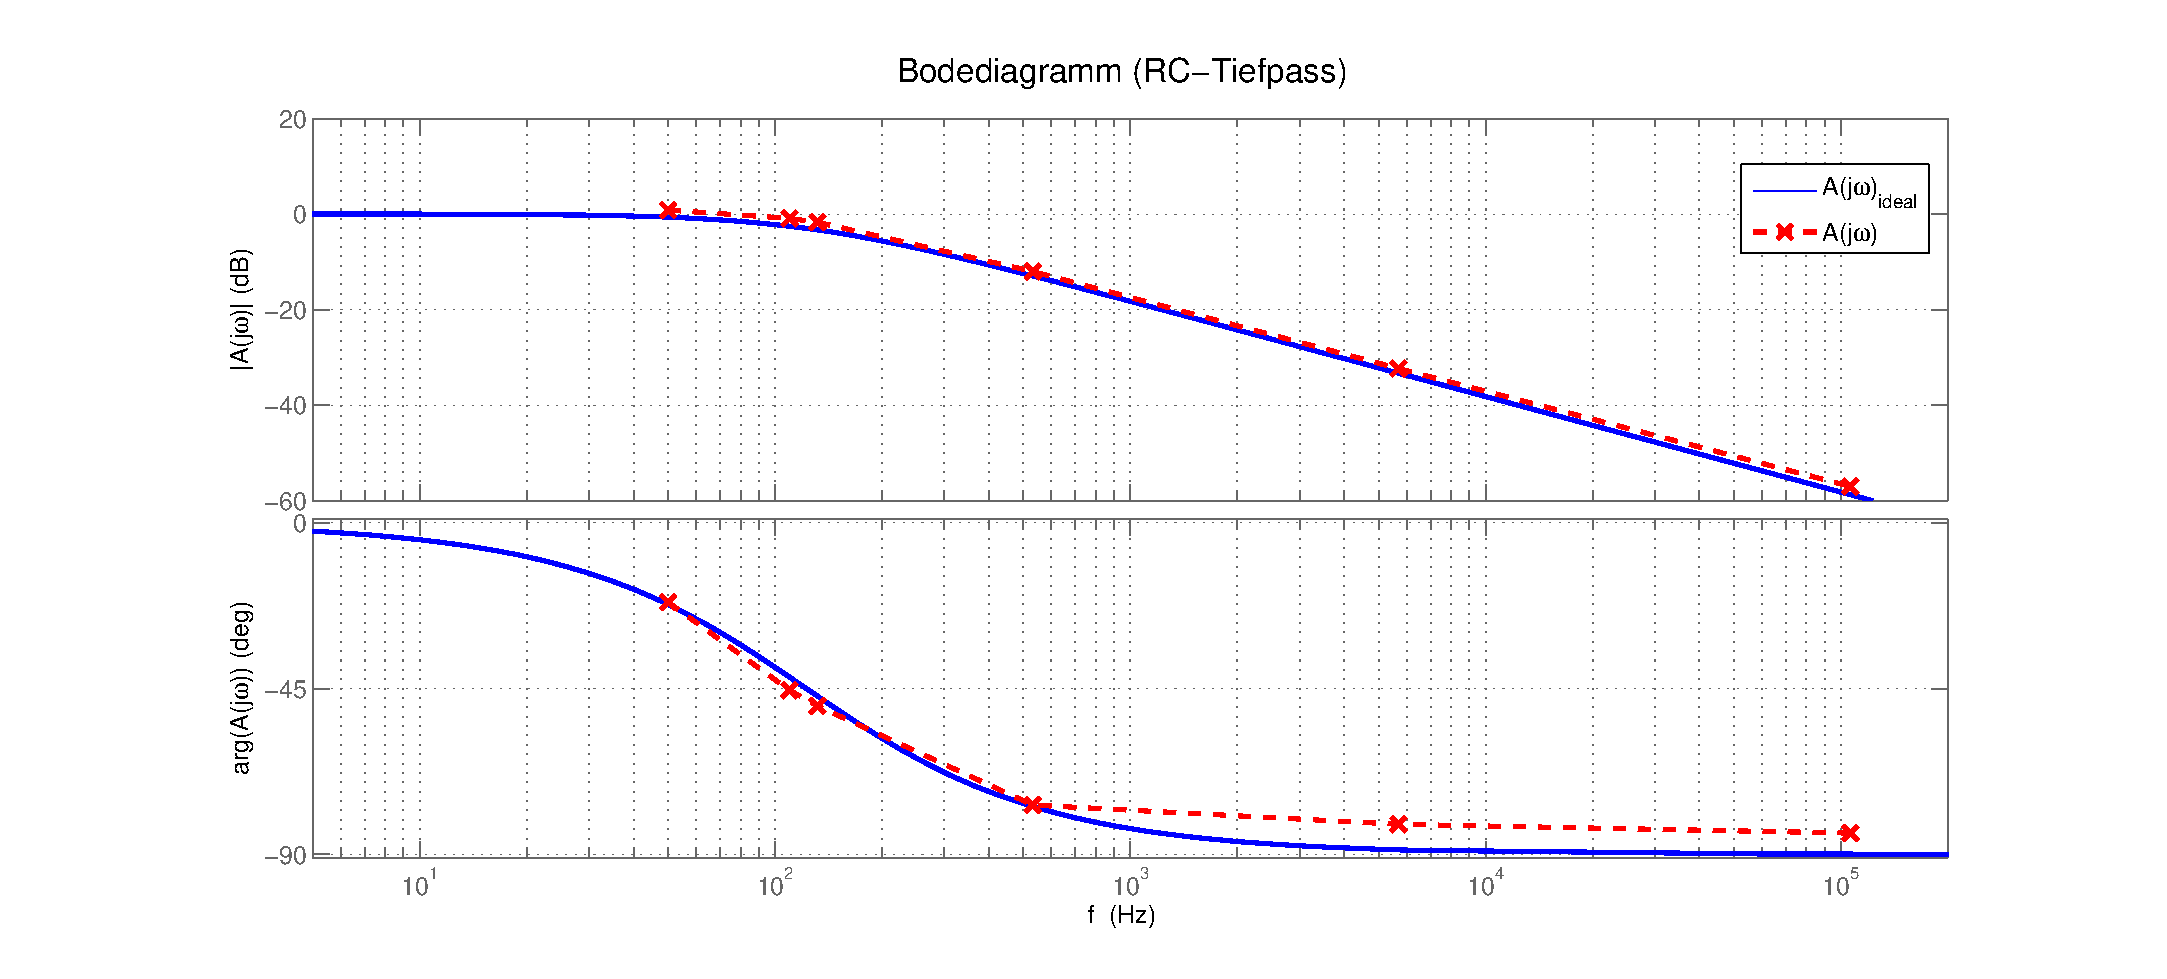
\includegraphics[width=1.1\textwidth]{figures/bode_rc.eps} 
\caption{Bodediagramm des bekannten RC-Tiefpass Filters mit idealer und gemessener Kennlinie.}
\label{fig:bode_bek}
\end{figure}


\subsection{Geräteliste}
Hier wurde wieder der AMREL FG-513 Funktionsgenerator und das Voltcraft 662 Oscilloskop verwendet.

\subsection{Diskussion}
In dieser Teilübung wurde für einen bekannten Filter (RC-Tiefpass) mit gegebenen Bauteilwerten
die Grenzfrequenz berechnet und gemessen. Die berechnete Grenzfrequenz betrug $f_g = 122.43Hz$. Die Grenzfrequenz wurde bei einer Ausgangsamplitude von 70.7\% der Eingangsamplitude gemessen. Dazu wurde das Oszilloskop und die Prozentskala auf diesem verwendet.\\
Weiters wurde ein Bodediagramm aufgenommen. Hierfür wurde die Phasenverschiebung und die Ausgangsamplitude bei verschiedenen Frequenzen aufgenommen. Wie aus Abbildung \ref{fig:bode_bek} zu entnehmen ist, liegen die von uns gemessenen Werte bis auf die Phasenverschiebung bei den letzten beiden Werten sehr gut auf der idealen Kurve.

%\begin{thebibliography}{9}

%\bibitem{skript}
 % Teresa Meier, Dipl.-Ing. Georg Egger, Dipl.-Ing. Dr Michael Gebhart\\
 % \emph{Übung C: RFID}\\
 % Technische Universität Graz
%\end{thebibliography}

 



   
\end{document}
